\documentclass[1p]{elsarticle_modified}
%\bibliographystyle{elsarticle-num}

%\usepackage[colorlinks]{hyperref}
%\usepackage{abbrmath_seonhwa} %\Abb, \Ascr, \Acal ,\Abf, \Afrak
\usepackage{amsfonts}
\usepackage{amssymb}
\usepackage{amsmath}
\usepackage{amsthm}
\usepackage{scalefnt}
\usepackage{amsbsy}
\usepackage{kotex}
\usepackage{caption}
\usepackage{subfig}
\usepackage{color}
\usepackage{graphicx}
\usepackage{xcolor} %% white, black, red, green, blue, cyan, magenta, yellow
\usepackage{float}
\usepackage{setspace}
\usepackage{hyperref}

\usepackage{tikz}
\usetikzlibrary{arrows}

\usepackage{multirow}
\usepackage{array} % fixed length table
\usepackage{hhline}

%%%%%%%%%%%%%%%%%%%%%
\makeatletter
\renewcommand*\env@matrix[1][\arraystretch]{%
	\edef\arraystretch{#1}%
	\hskip -\arraycolsep
	\let\@ifnextchar\new@ifnextchar
	\array{*\c@MaxMatrixCols c}}
\makeatother %https://tex.stackexchange.com/questions/14071/how-can-i-increase-the-line-spacing-in-a-matrix
%%%%%%%%%%%%%%%

\usepackage[normalem]{ulem}

\newcommand{\msout}[1]{\ifmmode\text{\sout{\ensuremath{#1}}}\else\sout{#1}\fi}
%SOURCE: \msout is \stkout macro in https://tex.stackexchange.com/questions/20609/strikeout-in-math-mode

\newcommand{\cancel}[1]{
	\ifmmode
	{\color{red}\msout{#1}}
	\else
	{\color{red}\sout{#1}}
	\fi
}

\newcommand{\add}[1]{
	{\color{blue}\uwave{#1}}
}

\newcommand{\replace}[2]{
	\ifmmode
	{\color{red}\msout{#1}}{\color{blue}\uwave{#2}}
	\else
	{\color{red}\sout{#1}}{\color{blue}\uwave{#2}}
	\fi
}

\newcommand{\Sol}{\mathcal{S}} %segment
\newcommand{\D}{D} %diagram
\newcommand{\A}{\mathcal{A}} %arc


%%%%%%%%%%%%%%%%%%%%%%%%%%%%%5 test

\def\sl{\operatorname{\textup{SL}}(2,\Cbb)}
\def\psl{\operatorname{\textup{PSL}}(2,\Cbb)}
\def\quan{\mkern 1mu \triangleright \mkern 1mu}

\theoremstyle{definition}
\newtheorem{thm}{Theorem}[section]
\newtheorem{prop}[thm]{Proposition}
\newtheorem{lem}[thm]{Lemma}
\newtheorem{ques}[thm]{Question}
\newtheorem{cor}[thm]{Corollary}
\newtheorem{defn}[thm]{Definition}
\newtheorem{exam}[thm]{Example}
\newtheorem{rmk}[thm]{Remark}
\newtheorem{alg}[thm]{Algorithm}

\newcommand{\I}{\sqrt{-1}}
\begin{document}

%\begin{frontmatter}
%
%\title{Boundary parabolic representations of knots up to 8 crossings}
%
%%% Group authors per affiliation:
%\author{Yunhi Cho} 
%\address{Department of Mathematics, University of Seoul, Seoul, Korea}
%\ead{yhcho@uos.ac.kr}
%
%
%\author{Seonhwa Kim} %\fnref{s_kim}}
%\address{Center for Geometry and Physics, Institute for Basic Science, Pohang, 37673, Korea}
%\ead{ryeona17@ibs.re.kr}
%
%\author{Hyuk Kim}
%\address{Department of Mathematical Sciences, Seoul National University, Seoul 08826, Korea}
%\ead{hyukkim@snu.ac.kr}
%
%\author{Seokbeom Yoon}
%\address{Department of Mathematical Sciences, Seoul National University, Seoul, 08826,  Korea}
%\ead{sbyoon15@snu.ac.kr}
%
%\begin{abstract}
%We find all boundary parabolic representation of knots up to 8 crossings.
%
%\end{abstract}
%\begin{keyword}
%    \MSC[2010] 57M25 
%\end{keyword}
%
%\end{frontmatter}

%\linenumbers
%\tableofcontents
%
\newcommand\colored[1]{\textcolor{white}{\rule[-0.35ex]{0.8em}{1.4ex}}\kern-0.8em\color{red} #1}%
%\newcommand\colored[1]{\textcolor{white}{ #1}\kern-2.17ex	\textcolor{white}{ #1}\kern-1.81ex	\textcolor{white}{ #1}\kern-2.15ex\color{red}#1	}

{\Large $\underline{12n_{0775}~(K12n_{0775})}$}

\setlength{\tabcolsep}{10pt}
\renewcommand{\arraystretch}{1.6}
\vspace{1cm}\begin{tabular}{m{100pt}>{\centering\arraybackslash}m{274pt}}
\multirow{5}{120pt}{
	\centering
	\includegraphics[width=112pt]{../../../GIT/diagram.site/Diagrams/png/2864_12n_0775.png}\\
\ \ \ A knot diagram\footnotemark}&
\allowdisplaybreaks
\textbf{Linearized knot diagam} \\
\cline{2-2}
 &
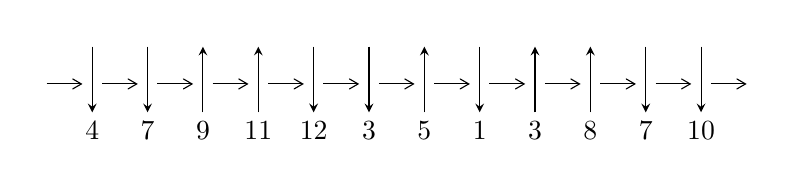
\begin{tikzpicture}[x=20pt, y=17pt]
	% nodes
	\node (C0) at (0, 0) {};
	\node (C1) at (1, 0) {};
	\node (C1U) at (1, +1) {};
	\node (C1D) at (1, -1) {4};

	\node (C2) at (2, 0) {};
	\node (C2U) at (2, +1) {};
	\node (C2D) at (2, -1) {7};

	\node (C3) at (3, 0) {};
	\node (C3U) at (3, +1) {};
	\node (C3D) at (3, -1) {9};

	\node (C4) at (4, 0) {};
	\node (C4U) at (4, +1) {};
	\node (C4D) at (4, -1) {11};

	\node (C5) at (5, 0) {};
	\node (C5U) at (5, +1) {};
	\node (C5D) at (5, -1) {12};

	\node (C6) at (6, 0) {};
	\node (C6U) at (6, +1) {};
	\node (C6D) at (6, -1) {3};

	\node (C7) at (7, 0) {};
	\node (C7U) at (7, +1) {};
	\node (C7D) at (7, -1) {5};

	\node (C8) at (8, 0) {};
	\node (C8U) at (8, +1) {};
	\node (C8D) at (8, -1) {1};

	\node (C9) at (9, 0) {};
	\node (C9U) at (9, +1) {};
	\node (C9D) at (9, -1) {3};

	\node (C10) at (10, 0) {};
	\node (C10U) at (10, +1) {};
	\node (C10D) at (10, -1) {8};

	\node (C11) at (11, 0) {};
	\node (C11U) at (11, +1) {};
	\node (C11D) at (11, -1) {7};

	\node (C12) at (12, 0) {};
	\node (C12U) at (12, +1) {};
	\node (C12D) at (12, -1) {10};
	\node (C13) at (13, 0) {};

	% arrows
	\draw[->,>={angle 60}]
	(C0) edge (C1) (C1) edge (C2) (C2) edge (C3) (C3) edge (C4) (C4) edge (C5) (C5) edge (C6) (C6) edge (C7) (C7) edge (C8) (C8) edge (C9) (C9) edge (C10) (C10) edge (C11) (C11) edge (C12) (C12) edge (C13) ;	\draw[->,>=stealth]
	(C1U) edge (C1D) (C2U) edge (C2D) (C3D) edge (C3U) (C4D) edge (C4U) (C5U) edge (C5D) (C6U) edge (C6D) (C7D) edge (C7U) (C8U) edge (C8D) (C9D) edge (C9U) (C10D) edge (C10U) (C11U) edge (C11D) (C12U) edge (C12D) ;
	\end{tikzpicture} \\
\hhline{~~} \\& 
\textbf{Solving Sequence} \\ \cline{2-2} 
 &
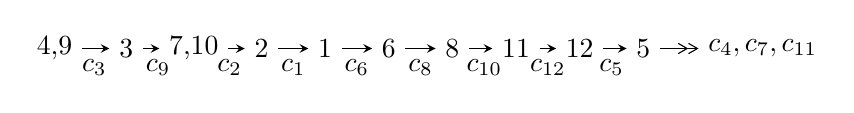
\begin{tikzpicture}[x=23pt, y=7pt]
	% node
	\node (A0) at (-1/8, 0) {4,9};
	\node (A1) at (1, 0) {3};
	\node (A2) at (33/16, 0) {7,10};
	\node (A3) at (25/8, 0) {2};
	\node (A4) at (33/8, 0) {1};
	\node (A5) at (41/8, 0) {6};
	\node (A6) at (49/8, 0) {8};
	\node (A7) at (57/8, 0) {11};
	\node (A8) at (65/8, 0) {12};
	\node (A9) at (73/8, 0) {5};
	\node (C1) at (1/2, -1) {$c_{3}$};
	\node (C2) at (3/2, -1) {$c_{9}$};
	\node (C3) at (21/8, -1) {$c_{2}$};
	\node (C4) at (29/8, -1) {$c_{1}$};
	\node (C5) at (37/8, -1) {$c_{6}$};
	\node (C6) at (45/8, -1) {$c_{8}$};
	\node (C7) at (53/8, -1) {$c_{10}$};
	\node (C8) at (61/8, -1) {$c_{12}$};
	\node (C9) at (69/8, -1) {$c_{5}$};
	\node (A10) at (11, 0) {$c_{4},c_{7},c_{11}$};

	% edge
	\draw[->,>=stealth]	
	(A0) edge (A1) (A1) edge (A2) (A2) edge (A3) (A3) edge (A4) (A4) edge (A5) (A5) edge (A6) (A6) edge (A7) (A7) edge (A8) (A8) edge (A9) ;
	\draw[->>,>={angle 60}]	
	(A9) edge (A10);
\end{tikzpicture} \\ 

\end{tabular} \\

\footnotetext{
The image of knot diagram is generated by the software ``\textbf{Draw programme}" developed by Andrew Bartholomew(\url{http://www.layer8.co.uk/maths/draw/index.htm\#Running-draw}), where we modified some parts for our purpose(\url{https://github.com/CATsTAILs/LinksPainter}).
}\phantom \\ \newline 
\centering \textbf{Ideals for irreducible components\footnotemark of $X_{\text{par}}$} 
 
\begin{align*}
I^u_{1}&=\langle 
4.72946\times10^{550} u^{111}+2.16316\times10^{551} u^{110}+\cdots+4.92224\times10^{554} b-1.20545\times10^{554},\\
\phantom{I^u_{1}}&\phantom{= \langle  }-9.48171\times10^{554} u^{111}-4.01791\times10^{555} u^{110}+\cdots+3.37616\times10^{558} a+3.78754\times10^{559},\\
\phantom{I^u_{1}}&\phantom{= \langle  }u^{112}+4 u^{111}+\cdots-58325 u-6859\rangle \\
I^u_{2}&=\langle 
6.07912\times10^{52} u^{46}+2.17727\times10^{53} u^{45}+\cdots+2.21125\times10^{51} b-7.40591\times10^{51},\\
\phantom{I^u_{2}}&\phantom{= \langle  }-9.90092\times10^{52} u^{46}-3.59271\times10^{53} u^{45}+\cdots+2.21125\times10^{51} a+1.90357\times10^{52},\;u^{47}+3 u^{46}+\cdots+2 u+1\rangle \\
\\
\end{align*}
\raggedright * 2 irreducible components of $\dim_{\mathbb{C}}=0$, with total 159 representations.\\
\footnotetext{All coefficients of polynomials are rational numbers. But the coefficients are sometimes approximated in decimal forms when there is not enough margin.}
\newpage
\renewcommand{\arraystretch}{1}
\centering \section*{I. $I^u_{1}= \langle 4.73\times10^{550} u^{111}+2.16\times10^{551} u^{110}+\cdots+4.92\times10^{554} b-1.21\times10^{554},\;-9.48\times10^{554} u^{111}-4.02\times10^{555} u^{110}+\cdots+3.38\times10^{558} a+3.79\times10^{559},\;u^{112}+4 u^{111}+\cdots-58325 u-6859 \rangle$}
\flushleft \textbf{(i) Arc colorings}\\
\begin{tabular}{m{7pt} m{180pt} m{7pt} m{180pt} }
\flushright $a_{4}=$&$\begin{pmatrix}1\\0\end{pmatrix}$ \\
\flushright $a_{9}=$&$\begin{pmatrix}0\\u\end{pmatrix}$ \\
\flushright $a_{3}=$&$\begin{pmatrix}1\\u^2\end{pmatrix}$ \\
\flushright $a_{7}=$&$\begin{pmatrix}0.000280843 u^{111}+0.00119008 u^{110}+\cdots-32.1239 u-11.2185\\-0.0000960836 u^{111}-0.000439467 u^{110}+\cdots+4.92015 u+0.244899\end{pmatrix}$ \\
\flushright $a_{10}=$&$\begin{pmatrix}u\\u^3+u\end{pmatrix}$ \\
\flushright $a_{2}=$&$\begin{pmatrix}-0.000138137 u^{111}-0.000302670 u^{110}+\cdots+2.66029 u-2.85809\\5.61677\times10^{-6} u^{111}-0.0000925256 u^{110}+\cdots+11.2653 u+1.87081\end{pmatrix}$ \\
\flushright $a_{1}=$&$\begin{pmatrix}-0.000132520 u^{111}-0.000395196 u^{110}+\cdots+13.9256 u-0.987279\\5.61677\times10^{-6} u^{111}-0.0000925256 u^{110}+\cdots+11.2653 u+1.87081\end{pmatrix}$ \\
\flushright $a_{6}=$&$\begin{pmatrix}0.000313936 u^{111}+0.00143159 u^{110}+\cdots-33.0210 u-11.4311\\-0.000175323 u^{111}-0.000907347 u^{110}+\cdots+11.5124 u+0.993446\end{pmatrix}$ \\
\flushright $a_{8}=$&$\begin{pmatrix}-0.000245594 u^{111}-0.000947597 u^{110}+\cdots+34.1586 u+7.91000\\0.000161105 u^{111}+0.000657051 u^{110}+\cdots-4.86191 u-0.127743\end{pmatrix}$ \\
\flushright $a_{11}=$&$\begin{pmatrix}0.000328032 u^{111}+0.00138695 u^{110}+\cdots-39.0729 u-7.92306\\-0.0000170292 u^{111}-0.000100765 u^{110}+\cdots+0.692184 u-0.497656\end{pmatrix}$ \\
\flushright $a_{12}=$&$\begin{pmatrix}-0.000127367 u^{111}-0.000200399 u^{110}+\cdots+4.99895 u-2.21822\\-0.0000483797 u^{111}-0.000392963 u^{110}+\cdots+12.5333 u+1.83459\end{pmatrix}$ \\
\flushright $a_{5}=$&$\begin{pmatrix}0.000227088 u^{111}+0.000766160 u^{110}+\cdots-1.60868 u-2.46399\\-0.0000568114 u^{111}-0.000133618 u^{110}+\cdots-5.98721 u-0.924727\end{pmatrix}$\\&\end{tabular}
\flushleft \textbf{(ii) Obstruction class $= -1$}\\~\\
\flushleft \textbf{(iii) Cusp Shapes $= 0.000127691 u^{111}+0.000648814 u^{110}+\cdots-28.0526 u+4.80987$}\\~\\
\newpage\renewcommand{\arraystretch}{1}
\flushleft \textbf{(iv) u-Polynomials at the component}\newline \\
\begin{tabular}{m{50pt}|m{274pt}}
Crossings & \hspace{64pt}u-Polynomials at each crossing \\
\hline $$\begin{aligned}c_{1}\end{aligned}$$&$\begin{aligned}
&u^{112}-9 u^{111}+\cdots-8787594026 u+1142120643
\end{aligned}$\\
\hline $$\begin{aligned}c_{2},c_{6}\end{aligned}$$&$\begin{aligned}
&u^{112}+4 u^{111}+\cdots-15875381 u-1020181
\end{aligned}$\\
\hline $$\begin{aligned}c_{3},c_{9}\end{aligned}$$&$\begin{aligned}
&u^{112}+4 u^{111}+\cdots-58325 u-6859
\end{aligned}$\\
\hline $$\begin{aligned}c_{4}\end{aligned}$$&$\begin{aligned}
&u^{112}+3 u^{111}+\cdots-55496 u-8997
\end{aligned}$\\
\hline $$\begin{aligned}c_{5}\end{aligned}$$&$\begin{aligned}
&u^{112}- u^{111}+\cdots-458318546098 u+137795579005
\end{aligned}$\\
\hline $$\begin{aligned}c_{7}\end{aligned}$$&$\begin{aligned}
&u^{112}+6 u^{111}+\cdots+437 u+19
\end{aligned}$\\
\hline $$\begin{aligned}c_{8}\end{aligned}$$&$\begin{aligned}
&u^{112}+u^{111}+\cdots-85 u-1
\end{aligned}$\\
\hline $$\begin{aligned}c_{10}\end{aligned}$$&$\begin{aligned}
&u^{112}-3 u^{111}+\cdots+13903468 u+3529277
\end{aligned}$\\
\hline $$\begin{aligned}c_{11}\end{aligned}$$&$\begin{aligned}
&u^{112}-7 u^{111}+\cdots+8027953 u+4448443
\end{aligned}$\\
\hline $$\begin{aligned}c_{12}\end{aligned}$$&$\begin{aligned}
&u^{112}+4 u^{111}+\cdots+29852667 u+2796781
\end{aligned}$\\
\hline
\end{tabular}\\~\\
\newpage\renewcommand{\arraystretch}{1}
\flushleft \textbf{(v) Riley Polynomials at the component}\newline \\
\begin{tabular}{m{50pt}|m{274pt}}
Crossings & \hspace{64pt}Riley Polynomials at each crossing \\
\hline $$\begin{aligned}c_{1}\end{aligned}$$&$\begin{aligned}
&y^{112}-75 y^{111}+\cdots-1.37\times10^{19} y+1.30\times10^{18}
\end{aligned}$\\
\hline $$\begin{aligned}c_{2},c_{6}\end{aligned}$$&$\begin{aligned}
&y^{112}-112 y^{111}+\cdots+38800688855225 y+1040769272761
\end{aligned}$\\
\hline $$\begin{aligned}c_{3},c_{9}\end{aligned}$$&$\begin{aligned}
&y^{112}+78 y^{111}+\cdots-34516755 y+47045881
\end{aligned}$\\
\hline $$\begin{aligned}c_{4}\end{aligned}$$&$\begin{aligned}
&y^{112}+31 y^{111}+\cdots+1564391402 y+80946009
\end{aligned}$\\
\hline $$\begin{aligned}c_{5}\end{aligned}$$&$\begin{aligned}
&y^{112}-55 y^{111}+\cdots+9.87\times10^{22} y+1.90\times10^{22}
\end{aligned}$\\
\hline $$\begin{aligned}c_{7}\end{aligned}$$&$\begin{aligned}
&y^{112}-2 y^{111}+\cdots-23009 y+361
\end{aligned}$\\
\hline $$\begin{aligned}c_{8}\end{aligned}$$&$\begin{aligned}
&y^{112}-7 y^{111}+\cdots+15211 y+1
\end{aligned}$\\
\hline $$\begin{aligned}c_{10}\end{aligned}$$&$\begin{aligned}
&y^{112}-17 y^{111}+\cdots+813550693297028 y+12455796142729
\end{aligned}$\\
\hline $$\begin{aligned}c_{11}\end{aligned}$$&$\begin{aligned}
&y^{112}-101 y^{111}+\cdots+1303442294494373 y+19788645124249
\end{aligned}$\\
\hline $$\begin{aligned}c_{12}\end{aligned}$$&$\begin{aligned}
&y^{112}-50 y^{111}+\cdots+1010612326184383 y+7821983961961
\end{aligned}$\\
\hline
\end{tabular}\\~\\
\newpage\flushleft \textbf{(vi) Complex Volumes and Cusp Shapes}
$$\begin{array}{c|c|c}  
\text{Solutions to }I^u_{1}& \I (\text{vol} + \sqrt{-1}CS) & \text{Cusp shape}\\
 \hline 
\begin{aligned}
u &= \phantom{-}0.820472 + 0.562696 I \\
a &= -0.610188 + 0.796078 I \\
b &= \phantom{-}0.749858 - 0.604560 I\end{aligned}
 & -4.54077 - 2.35893 I & \phantom{-0.000000 } 0 \\ \hline\begin{aligned}
u &= \phantom{-}0.820472 - 0.562696 I \\
a &= -0.610188 - 0.796078 I \\
b &= \phantom{-}0.749858 + 0.604560 I\end{aligned}
 & -4.54077 + 2.35893 I & \phantom{-0.000000 } 0 \\ \hline\begin{aligned}
u &= \phantom{-}0.192272 + 0.988334 I \\
a &= \phantom{-}0.134561 + 1.314880 I \\
b &= -0.360895 + 0.348983 I\end{aligned}
 & \phantom{-}4.95567 + 0.74367 I & \phantom{-0.000000 } 0 \\ \hline\begin{aligned}
u &= \phantom{-}0.192272 - 0.988334 I \\
a &= \phantom{-}0.134561 - 1.314880 I \\
b &= -0.360895 - 0.348983 I\end{aligned}
 & \phantom{-}4.95567 - 0.74367 I & \phantom{-0.000000 } 0 \\ \hline\begin{aligned}
u &= \phantom{-}0.683818 + 0.687327 I \\
a &= \phantom{-}0.166713 - 0.372936 I \\
b &= -0.330665 - 0.119114 I\end{aligned}
 & \phantom{-}1.37759 + 2.46422 I & \phantom{-0.000000 } 0 \\ \hline\begin{aligned}
u &= \phantom{-}0.683818 - 0.687327 I \\
a &= \phantom{-}0.166713 + 0.372936 I \\
b &= -0.330665 + 0.119114 I\end{aligned}
 & \phantom{-}1.37759 - 2.46422 I & \phantom{-0.000000 } 0 \\ \hline\begin{aligned}
u &= \phantom{-}0.515372 + 0.912803 I \\
a &= \phantom{-}0.42132 - 1.50020 I \\
b &= -0.323125 + 1.248830 I\end{aligned}
 & -5.60049 + 7.43511 I & \phantom{-0.000000 } 0 \\ \hline\begin{aligned}
u &= \phantom{-}0.515372 - 0.912803 I \\
a &= \phantom{-}0.42132 + 1.50020 I \\
b &= -0.323125 - 1.248830 I\end{aligned}
 & -5.60049 - 7.43511 I & \phantom{-0.000000 } 0 \\ \hline\begin{aligned}
u &= -0.251961 + 0.906396 I \\
a &= \phantom{-}0.76478 - 1.54270 I \\
b &= -1.165860 - 0.019395 I\end{aligned}
 & \phantom{-}2.58226 - 1.11403 I & \phantom{-0.000000 } 0 \\ \hline\begin{aligned}
u &= -0.251961 - 0.906396 I \\
a &= \phantom{-}0.76478 + 1.54270 I \\
b &= -1.165860 + 0.019395 I\end{aligned}
 & \phantom{-}2.58226 + 1.11403 I & \phantom{-0.000000 } 0\\
 \hline 
 \end{array}$$\newpage$$\begin{array}{c|c|c}  
\text{Solutions to }I^u_{1}& \I (\text{vol} + \sqrt{-1}CS) & \text{Cusp shape}\\
 \hline 
\begin{aligned}
u &= -0.230071 + 0.883448 I \\
a &= \phantom{-}0.055779 - 0.188613 I \\
b &= \phantom{-}0.757231 + 0.273492 I\end{aligned}
 & -3.63124 + 0.79197 I & \phantom{-0.000000 } 0 \\ \hline\begin{aligned}
u &= -0.230071 - 0.883448 I \\
a &= \phantom{-}0.055779 + 0.188613 I \\
b &= \phantom{-}0.757231 - 0.273492 I\end{aligned}
 & -3.63124 - 0.79197 I & \phantom{-0.000000 } 0 \\ \hline\begin{aligned}
u &= -0.625382 + 0.892347 I \\
a &= \phantom{-}1.43689 - 1.91980 I \\
b &= -2.45987 + 0.62363 I\end{aligned}
 & \phantom{-}4.79451 - 2.46272 I & \phantom{-0.000000 } 0 \\ \hline\begin{aligned}
u &= -0.625382 - 0.892347 I \\
a &= \phantom{-}1.43689 + 1.91980 I \\
b &= -2.45987 - 0.62363 I\end{aligned}
 & \phantom{-}4.79451 + 2.46272 I & \phantom{-0.000000 } 0 \\ \hline\begin{aligned}
u &= \phantom{-}0.535431 + 0.976259 I \\
a &= \phantom{-}0.220208 + 0.415433 I \\
b &= -0.145589 - 0.236451 I\end{aligned}
 & \phantom{-}0.39793 + 2.25572 I & \phantom{-0.000000 } 0 \\ \hline\begin{aligned}
u &= \phantom{-}0.535431 - 0.976259 I \\
a &= \phantom{-}0.220208 - 0.415433 I \\
b &= -0.145589 + 0.236451 I\end{aligned}
 & \phantom{-}0.39793 - 2.25572 I & \phantom{-0.000000 } 0 \\ \hline\begin{aligned}
u &= \phantom{-}0.370960 + 1.052540 I \\
a &= -1.314470 + 0.505056 I \\
b &= \phantom{-}0.96982 - 1.30873 I\end{aligned}
 & -3.79912 + 5.92613 I & \phantom{-0.000000 } 0 \\ \hline\begin{aligned}
u &= \phantom{-}0.370960 - 1.052540 I \\
a &= -1.314470 - 0.505056 I \\
b &= \phantom{-}0.96982 + 1.30873 I\end{aligned}
 & -3.79912 - 5.92613 I & \phantom{-0.000000 } 0 \\ \hline\begin{aligned}
u &= -0.810666 + 0.304232 I \\
a &= \phantom{-}0.046719 - 0.197447 I \\
b &= \phantom{-}1.208720 - 0.245075 I\end{aligned}
 & -3.14523 + 0.13283 I & \phantom{-0.000000 } 0 \\ \hline\begin{aligned}
u &= -0.810666 - 0.304232 I \\
a &= \phantom{-}0.046719 + 0.197447 I \\
b &= \phantom{-}1.208720 + 0.245075 I\end{aligned}
 & -3.14523 - 0.13283 I & \phantom{-0.000000 } 0\\
 \hline 
 \end{array}$$\newpage$$\begin{array}{c|c|c}  
\text{Solutions to }I^u_{1}& \I (\text{vol} + \sqrt{-1}CS) & \text{Cusp shape}\\
 \hline 
\begin{aligned}
u &= -0.029973 + 1.144160 I \\
a &= \phantom{-}0.904002 - 0.401965 I \\
b &= -0.55721 + 1.38898 I\end{aligned}
 & -2.17519 - 5.17005 I & \phantom{-0.000000 } 0 \\ \hline\begin{aligned}
u &= -0.029973 - 1.144160 I \\
a &= \phantom{-}0.904002 + 0.401965 I \\
b &= -0.55721 - 1.38898 I\end{aligned}
 & -2.17519 + 5.17005 I & \phantom{-0.000000 } 0 \\ \hline\begin{aligned}
u &= -0.760594 + 0.373854 I \\
a &= \phantom{-}0.191943 - 0.611863 I \\
b &= -0.070552 - 0.361483 I\end{aligned}
 & \phantom{-}0.05174 + 3.76897 I & \phantom{-0.000000 } 0 \\ \hline\begin{aligned}
u &= -0.760594 - 0.373854 I \\
a &= \phantom{-}0.191943 + 0.611863 I \\
b &= -0.070552 + 0.361483 I\end{aligned}
 & \phantom{-}0.05174 - 3.76897 I & \phantom{-0.000000 } 0 \\ \hline\begin{aligned}
u &= -0.459153 + 1.057810 I \\
a &= -0.79656 + 1.24755 I \\
b &= \phantom{-}0.692312 - 0.581892 I\end{aligned}
 & -5.26545 - 4.52408 I & \phantom{-0.000000 } 0 \\ \hline\begin{aligned}
u &= -0.459153 - 1.057810 I \\
a &= -0.79656 - 1.24755 I \\
b &= \phantom{-}0.692312 + 0.581892 I\end{aligned}
 & -5.26545 + 4.52408 I & \phantom{-0.000000 } 0 \\ \hline\begin{aligned}
u &= \phantom{-}1.044220 + 0.536131 I \\
a &= \phantom{-}0.130077 + 1.360110 I \\
b &= -1.021250 - 0.147732 I\end{aligned}
 & \phantom{-}0.14579 + 5.18168 I & \phantom{-0.000000 } 0 \\ \hline\begin{aligned}
u &= \phantom{-}1.044220 - 0.536131 I \\
a &= \phantom{-}0.130077 - 1.360110 I \\
b &= -1.021250 + 0.147732 I\end{aligned}
 & \phantom{-}0.14579 - 5.18168 I & \phantom{-0.000000 } 0 \\ \hline\begin{aligned}
u &= -0.126808 + 0.779708 I \\
a &= \phantom{-}0.25097 + 1.83833 I \\
b &= -0.355896 - 0.381890 I\end{aligned}
 & -0.86855 + 4.51509 I & \phantom{-0.000000 } 0 \\ \hline\begin{aligned}
u &= -0.126808 - 0.779708 I \\
a &= \phantom{-}0.25097 - 1.83833 I \\
b &= -0.355896 + 0.381890 I\end{aligned}
 & -0.86855 - 4.51509 I & \phantom{-0.000000 } 0\\
 \hline 
 \end{array}$$\newpage$$\begin{array}{c|c|c}  
\text{Solutions to }I^u_{1}& \I (\text{vol} + \sqrt{-1}CS) & \text{Cusp shape}\\
 \hline 
\begin{aligned}
u &= -0.482246 + 0.610736 I \\
a &= -0.335837 + 0.313447 I \\
b &= \phantom{-}1.389450 - 0.115206 I\end{aligned}
 & -3.36847 + 0.61627 I & \phantom{-0.000000 } 0 \\ \hline\begin{aligned}
u &= -0.482246 - 0.610736 I \\
a &= -0.335837 - 0.313447 I \\
b &= \phantom{-}1.389450 + 0.115206 I\end{aligned}
 & -3.36847 - 0.61627 I & \phantom{-0.000000 } 0 \\ \hline\begin{aligned}
u &= -0.413576 + 1.156490 I \\
a &= -0.194129 + 0.092382 I \\
b &= \phantom{-}0.401166 + 0.631290 I\end{aligned}
 & -4.20708 - 6.00888 I & \phantom{-0.000000 } 0 \\ \hline\begin{aligned}
u &= -0.413576 - 1.156490 I \\
a &= -0.194129 - 0.092382 I \\
b &= \phantom{-}0.401166 - 0.631290 I\end{aligned}
 & -4.20708 + 6.00888 I & \phantom{-0.000000 } 0 \\ \hline\begin{aligned}
u &= -0.067809 + 1.235900 I \\
a &= -2.39842 + 0.29783 I \\
b &= \phantom{-}2.08495 - 0.10259 I\end{aligned}
 & -5.65446 - 2.17511 I & \phantom{-0.000000 } 0 \\ \hline\begin{aligned}
u &= -0.067809 - 1.235900 I \\
a &= -2.39842 - 0.29783 I \\
b &= \phantom{-}2.08495 + 0.10259 I\end{aligned}
 & -5.65446 + 2.17511 I & \phantom{-0.000000 } 0 \\ \hline\begin{aligned}
u &= -0.602494 + 1.083240 I \\
a &= -0.1057130 - 0.0812277 I \\
b &= -0.436934 + 0.197677 I\end{aligned}
 & -1.99769 - 8.93050 I & \phantom{-0.000000 } 0 \\ \hline\begin{aligned}
u &= -0.602494 - 1.083240 I \\
a &= -0.1057130 + 0.0812277 I \\
b &= -0.436934 - 0.197677 I\end{aligned}
 & -1.99769 + 8.93050 I & \phantom{-0.000000 } 0 \\ \hline\begin{aligned}
u &= -0.249742 + 1.234070 I \\
a &= -2.19288 + 0.51178 I \\
b &= \phantom{-}2.10567 + 0.54100 I\end{aligned}
 & -5.63157 - 3.78862 I & \phantom{-0.000000 } 0 \\ \hline\begin{aligned}
u &= -0.249742 - 1.234070 I \\
a &= -2.19288 - 0.51178 I \\
b &= \phantom{-}2.10567 - 0.54100 I\end{aligned}
 & -5.63157 + 3.78862 I & \phantom{-0.000000 } 0\\
 \hline 
 \end{array}$$\newpage$$\begin{array}{c|c|c}  
\text{Solutions to }I^u_{1}& \I (\text{vol} + \sqrt{-1}CS) & \text{Cusp shape}\\
 \hline 
\begin{aligned}
u &= \phantom{-}0.666204 + 1.070400 I \\
a &= \phantom{-}0.513000 + 0.183372 I \\
b &= -1.163080 - 0.268835 I\end{aligned}
 & -1.86055 + 1.14037 I & \phantom{-0.000000 } 0 \\ \hline\begin{aligned}
u &= \phantom{-}0.666204 - 1.070400 I \\
a &= \phantom{-}0.513000 - 0.183372 I \\
b &= -1.163080 + 0.268835 I\end{aligned}
 & -1.86055 - 1.14037 I & \phantom{-0.000000 } 0 \\ \hline\begin{aligned}
u &= -0.085971 + 1.263370 I \\
a &= \phantom{-}1.092920 + 0.492671 I \\
b &= -0.89546 - 1.54696 I\end{aligned}
 & -0.319616 - 0.226105 I & \phantom{-0.000000 } 0 \\ \hline\begin{aligned}
u &= -0.085971 - 1.263370 I \\
a &= \phantom{-}1.092920 - 0.492671 I \\
b &= -0.89546 + 1.54696 I\end{aligned}
 & -0.319616 + 0.226105 I & \phantom{-0.000000 } 0 \\ \hline\begin{aligned}
u &= -0.203736 + 1.268160 I \\
a &= -0.0034625 - 0.0350637 I \\
b &= \phantom{-}0.137235 + 0.814280 I\end{aligned}
 & -5.70721 - 0.73948 I & \phantom{-0.000000 } 0 \\ \hline\begin{aligned}
u &= -0.203736 - 1.268160 I \\
a &= -0.0034625 + 0.0350637 I \\
b &= \phantom{-}0.137235 - 0.814280 I\end{aligned}
 & -5.70721 + 0.73948 I & \phantom{-0.000000 } 0 \\ \hline\begin{aligned}
u &= -1.288250 + 0.075127 I \\
a &= \phantom{-}0.094427 - 0.327496 I \\
b &= \phantom{-}1.82157 - 0.04101 I\end{aligned}
 & -6.92130 - 3.75023 I & \phantom{-0.000000 } 0 \\ \hline\begin{aligned}
u &= -1.288250 - 0.075127 I \\
a &= \phantom{-}0.094427 + 0.327496 I \\
b &= \phantom{-}1.82157 + 0.04101 I\end{aligned}
 & -6.92130 + 3.75023 I & \phantom{-0.000000 } 0 \\ \hline\begin{aligned}
u &= -0.044785 + 1.300280 I \\
a &= \phantom{-}2.60956 + 0.17251 I \\
b &= -2.83914 - 0.48601 I\end{aligned}
 & -9.59880 - 6.71685 I & \phantom{-0.000000 } 0 \\ \hline\begin{aligned}
u &= -0.044785 - 1.300280 I \\
a &= \phantom{-}2.60956 - 0.17251 I \\
b &= -2.83914 + 0.48601 I\end{aligned}
 & -9.59880 + 6.71685 I & \phantom{-0.000000 } 0\\
 \hline 
 \end{array}$$\newpage$$\begin{array}{c|c|c}  
\text{Solutions to }I^u_{1}& \I (\text{vol} + \sqrt{-1}CS) & \text{Cusp shape}\\
 \hline 
\begin{aligned}
u &= -0.066281 + 1.303150 I \\
a &= -1.03065 - 1.21787 I \\
b &= \phantom{-}0.99259 + 2.58235 I\end{aligned}
 & -2.34168 - 6.96805 I & \phantom{-0.000000 } 0 \\ \hline\begin{aligned}
u &= -0.066281 - 1.303150 I \\
a &= -1.03065 + 1.21787 I \\
b &= \phantom{-}0.99259 - 2.58235 I\end{aligned}
 & -2.34168 + 6.96805 I & \phantom{-0.000000 } 0 \\ \hline\begin{aligned}
u &= -0.661126 + 0.186885 I \\
a &= \phantom{-}0.974380 + 0.107720 I \\
b &= \phantom{-}0.451910 - 0.045072 I\end{aligned}
 & -1.30680 + 1.95430 I & -2.00000 - 3.74794 I \\ \hline\begin{aligned}
u &= -0.661126 - 0.186885 I \\
a &= \phantom{-}0.974380 - 0.107720 I \\
b &= \phantom{-}0.451910 + 0.045072 I\end{aligned}
 & -1.30680 - 1.95430 I & -2.00000 + 3.74794 I \\ \hline\begin{aligned}
u &= -0.205430 + 1.314940 I \\
a &= \phantom{-}1.68962 - 0.69503 I \\
b &= -1.79990 + 0.80722 I\end{aligned}
 & -9.26055 - 4.29629 I & \phantom{-0.000000 } 0 \\ \hline\begin{aligned}
u &= -0.205430 - 1.314940 I \\
a &= \phantom{-}1.68962 + 0.69503 I \\
b &= -1.79990 - 0.80722 I\end{aligned}
 & -9.26055 + 4.29629 I & \phantom{-0.000000 } 0 \\ \hline\begin{aligned}
u &= \phantom{-}1.345730 + 0.066228 I \\
a &= \phantom{-}0.380481 - 0.166342 I \\
b &= \phantom{-}2.11618 - 0.08970 I\end{aligned}
 & -5.52257 + 1.61467 I & \phantom{-0.000000 } 0 \\ \hline\begin{aligned}
u &= \phantom{-}1.345730 - 0.066228 I \\
a &= \phantom{-}0.380481 + 0.166342 I \\
b &= \phantom{-}2.11618 + 0.08970 I\end{aligned}
 & -5.52257 - 1.61467 I & \phantom{-0.000000 } 0 \\ \hline\begin{aligned}
u &= \phantom{-}0.618605 + 0.165341 I \\
a &= \phantom{-}0.811260 - 0.887395 I \\
b &= \phantom{-}0.445574 + 0.782574 I\end{aligned}
 & -1.45852 - 2.39541 I & -2.76939 + 2.29844 I \\ \hline\begin{aligned}
u &= \phantom{-}0.618605 - 0.165341 I \\
a &= \phantom{-}0.811260 + 0.887395 I \\
b &= \phantom{-}0.445574 - 0.782574 I\end{aligned}
 & -1.45852 + 2.39541 I & -2.76939 - 2.29844 I\\
 \hline 
 \end{array}$$\newpage$$\begin{array}{c|c|c}  
\text{Solutions to }I^u_{1}& \I (\text{vol} + \sqrt{-1}CS) & \text{Cusp shape}\\
 \hline 
\begin{aligned}
u &= \phantom{-}0.253530 + 1.337200 I \\
a &= -1.82896 - 0.48628 I \\
b &= \phantom{-}1.65501 - 0.68419 I\end{aligned}
 & -6.63750 + 6.21609 I & \phantom{-0.000000 } 0 \\ \hline\begin{aligned}
u &= \phantom{-}0.253530 - 1.337200 I \\
a &= -1.82896 + 0.48628 I \\
b &= \phantom{-}1.65501 + 0.68419 I\end{aligned}
 & -6.63750 - 6.21609 I & \phantom{-0.000000 } 0 \\ \hline\begin{aligned}
u &= \phantom{-}0.285422 + 0.536350 I \\
a &= \phantom{-}1.40090 - 0.81746 I \\
b &= -0.035432 - 0.217193 I\end{aligned}
 & \phantom{-}0.82427 + 2.54264 I & \phantom{-}6.91993 - 6.04740 I \\ \hline\begin{aligned}
u &= \phantom{-}0.285422 - 0.536350 I \\
a &= \phantom{-}1.40090 + 0.81746 I \\
b &= -0.035432 + 0.217193 I\end{aligned}
 & \phantom{-}0.82427 - 2.54264 I & \phantom{-}6.91993 + 6.04740 I \\ \hline\begin{aligned}
u &= -1.382520 + 0.211454 I \\
a &= -0.37785 + 1.47718 I \\
b &= -0.09063 + 2.23933 I\end{aligned}
 & \phantom{-}5.13845 - 3.88562 I & \phantom{-0.000000 } 0 \\ \hline\begin{aligned}
u &= -1.382520 - 0.211454 I \\
a &= -0.37785 - 1.47718 I \\
b &= -0.09063 - 2.23933 I\end{aligned}
 & \phantom{-}5.13845 + 3.88562 I & \phantom{-0.000000 } 0 \\ \hline\begin{aligned}
u &= -1.402850 + 0.098193 I \\
a &= -0.104941 + 0.247776 I \\
b &= -1.90261 + 0.09484 I\end{aligned}
 & -7.42391 - 11.92370 I & \phantom{-0.000000 } 0 \\ \hline\begin{aligned}
u &= -1.402850 - 0.098193 I \\
a &= -0.104941 - 0.247776 I \\
b &= -1.90261 - 0.09484 I\end{aligned}
 & -7.42391 + 11.92370 I & \phantom{-0.000000 } 0 \\ \hline\begin{aligned}
u &= -0.143752 + 1.399190 I \\
a &= -1.68598 + 0.65970 I \\
b &= \phantom{-}2.26666 - 0.84935 I\end{aligned}
 & -9.27132 - 2.83279 I & \phantom{-0.000000 } 0 \\ \hline\begin{aligned}
u &= -0.143752 - 1.399190 I \\
a &= -1.68598 - 0.65970 I \\
b &= \phantom{-}2.26666 + 0.84935 I\end{aligned}
 & -9.27132 + 2.83279 I & \phantom{-0.000000 } 0\\
 \hline 
 \end{array}$$\newpage$$\begin{array}{c|c|c}  
\text{Solutions to }I^u_{1}& \I (\text{vol} + \sqrt{-1}CS) & \text{Cusp shape}\\
 \hline 
\begin{aligned}
u &= \phantom{-}0.258232 + 1.388350 I \\
a &= \phantom{-}0.463315 - 0.717360 I \\
b &= -0.234058 - 0.143351 I\end{aligned}
 & -6.36736 + 0.90340 I & \phantom{-0.000000 } 0 \\ \hline\begin{aligned}
u &= \phantom{-}0.258232 - 1.388350 I \\
a &= \phantom{-}0.463315 + 0.717360 I \\
b &= -0.234058 + 0.143351 I\end{aligned}
 & -6.36736 - 0.90340 I & \phantom{-0.000000 } 0 \\ \hline\begin{aligned}
u &= \phantom{-}0.17098 + 1.40758 I \\
a &= -0.239166 - 0.119759 I \\
b &= \phantom{-}0.042488 - 1.178640 I\end{aligned}
 & -2.11115 - 0.22606 I & \phantom{-0.000000 } 0 \\ \hline\begin{aligned}
u &= \phantom{-}0.17098 - 1.40758 I \\
a &= -0.239166 + 0.119759 I \\
b &= \phantom{-}0.042488 + 1.178640 I\end{aligned}
 & -2.11115 + 0.22606 I & \phantom{-0.000000 } 0 \\ \hline\begin{aligned}
u &= \phantom{-}0.537253 + 0.222267 I \\
a &= \phantom{-}1.48340 + 0.50119 I \\
b &= \phantom{-}1.38375 + 0.34335 I\end{aligned}
 & -2.75015 - 3.14737 I & -0.51905 + 9.05080 I \\ \hline\begin{aligned}
u &= \phantom{-}0.537253 - 0.222267 I \\
a &= \phantom{-}1.48340 - 0.50119 I \\
b &= \phantom{-}1.38375 - 0.34335 I\end{aligned}
 & -2.75015 + 3.14737 I & -0.51905 - 9.05080 I \\ \hline\begin{aligned}
u &= \phantom{-}0.20915 + 1.40309 I \\
a &= \phantom{-}1.77505 + 0.11194 I \\
b &= -1.59384 - 0.09968 I\end{aligned}
 & -11.3422 + 9.1428 I & \phantom{-0.000000 } 0 \\ \hline\begin{aligned}
u &= \phantom{-}0.20915 - 1.40309 I \\
a &= \phantom{-}1.77505 - 0.11194 I \\
b &= -1.59384 + 0.09968 I\end{aligned}
 & -11.3422 - 9.1428 I & \phantom{-0.000000 } 0 \\ \hline\begin{aligned}
u &= \phantom{-}0.208395 + 0.532517 I \\
a &= \phantom{-}0.682181 + 0.441617 I \\
b &= \phantom{-}0.041881 - 0.377150 I\end{aligned}
 & -0.144616 + 1.089290 I & -2.18626 - 6.39033 I \\ \hline\begin{aligned}
u &= \phantom{-}0.208395 - 0.532517 I \\
a &= \phantom{-}0.682181 - 0.441617 I \\
b &= \phantom{-}0.041881 + 0.377150 I\end{aligned}
 & -0.144616 - 1.089290 I & -2.18626 + 6.39033 I\\
 \hline 
 \end{array}$$\newpage$$\begin{array}{c|c|c}  
\text{Solutions to }I^u_{1}& \I (\text{vol} + \sqrt{-1}CS) & \text{Cusp shape}\\
 \hline 
\begin{aligned}
u &= \phantom{-}0.02898 + 1.43111 I \\
a &= \phantom{-}1.82656 - 0.02849 I \\
b &= -1.82470 + 0.47918 I\end{aligned}
 & -10.80120 + 1.32037 I & \phantom{-0.000000 } 0 \\ \hline\begin{aligned}
u &= \phantom{-}0.02898 - 1.43111 I \\
a &= \phantom{-}1.82656 + 0.02849 I \\
b &= -1.82470 - 0.47918 I\end{aligned}
 & -10.80120 - 1.32037 I & \phantom{-0.000000 } 0 \\ \hline\begin{aligned}
u &= \phantom{-}0.15091 + 1.49713 I \\
a &= -1.57712 + 0.02312 I \\
b &= \phantom{-}1.61128 + 0.19967 I\end{aligned}
 & -11.68300 + 0.74838 I & \phantom{-0.000000 } 0 \\ \hline\begin{aligned}
u &= \phantom{-}0.15091 - 1.49713 I \\
a &= -1.57712 - 0.02312 I \\
b &= \phantom{-}1.61128 - 0.19967 I\end{aligned}
 & -11.68300 - 0.74838 I & \phantom{-0.000000 } 0 \\ \hline\begin{aligned}
u &= \phantom{-}0.27742 + 1.49925 I \\
a &= -0.448214 + 0.558318 I \\
b &= \phantom{-}0.382683 + 0.348317 I\end{aligned}
 & -6.62895 + 9.45962 I & \phantom{-0.000000 } 0 \\ \hline\begin{aligned}
u &= \phantom{-}0.27742 - 1.49925 I \\
a &= -0.448214 - 0.558318 I \\
b &= \phantom{-}0.382683 - 0.348317 I\end{aligned}
 & -6.62895 - 9.45962 I & \phantom{-0.000000 } 0 \\ \hline\begin{aligned}
u &= \phantom{-}0.044364 + 0.462759 I \\
a &= -0.53060 + 5.86267 I \\
b &= \phantom{-}0.10112 - 1.96818 I\end{aligned}
 & \phantom{-}0.91865 + 6.75705 I & \phantom{-}7.45079 - 10.28372 I \\ \hline\begin{aligned}
u &= \phantom{-}0.044364 - 0.462759 I \\
a &= -0.53060 - 5.86267 I \\
b &= \phantom{-}0.10112 + 1.96818 I\end{aligned}
 & \phantom{-}0.91865 - 6.75705 I & \phantom{-}7.45079 + 10.28372 I \\ \hline\begin{aligned}
u &= -0.57564 + 1.46674 I \\
a &= -1.55233 + 0.76795 I \\
b &= \phantom{-}2.32643 + 0.37954 I\end{aligned}
 & -11.7977 - 10.2663 I & \phantom{-0.000000 } 0 \\ \hline\begin{aligned}
u &= -0.57564 - 1.46674 I \\
a &= -1.55233 - 0.76795 I \\
b &= \phantom{-}2.32643 - 0.37954 I\end{aligned}
 & -11.7977 + 10.2663 I & \phantom{-0.000000 } 0\\
 \hline 
 \end{array}$$\newpage$$\begin{array}{c|c|c}  
\text{Solutions to }I^u_{1}& \I (\text{vol} + \sqrt{-1}CS) & \text{Cusp shape}\\
 \hline 
\begin{aligned}
u &= \phantom{-}0.55607 + 1.51761 I \\
a &= -1.38201 - 0.59027 I \\
b &= \phantom{-}2.16220 - 0.97168 I\end{aligned}
 & -10.65990 + 8.34282 I & \phantom{-0.000000 } 0 \\ \hline\begin{aligned}
u &= \phantom{-}0.55607 - 1.51761 I \\
a &= -1.38201 + 0.59027 I \\
b &= \phantom{-}2.16220 + 0.97168 I\end{aligned}
 & -10.65990 - 8.34282 I & \phantom{-0.000000 } 0 \\ \hline\begin{aligned}
u &= -0.59693 + 1.50465 I \\
a &= \phantom{-}1.46749 - 0.72531 I \\
b &= -2.32030 - 0.48441 I\end{aligned}
 & -12.5086 - 18.8463 I & \phantom{-0.000000 } 0 \\ \hline\begin{aligned}
u &= -0.59693 - 1.50465 I \\
a &= \phantom{-}1.46749 + 0.72531 I \\
b &= -2.32030 + 0.48441 I\end{aligned}
 & -12.5086 + 18.8463 I & \phantom{-0.000000 } 0 \\ \hline\begin{aligned}
u &= \phantom{-}0.59585 + 1.51780 I \\
a &= -1.37222 - 0.68797 I \\
b &= \phantom{-}2.46447 - 0.62689 I\end{aligned}
 & -10.26930 + 5.43551 I & \phantom{-0.000000 } 0 \\ \hline\begin{aligned}
u &= \phantom{-}0.59585 - 1.51780 I \\
a &= -1.37222 + 0.68797 I \\
b &= \phantom{-}2.46447 + 0.62689 I\end{aligned}
 & -10.26930 - 5.43551 I & \phantom{-0.000000 } 0 \\ \hline\begin{aligned}
u &= -0.345280 + 0.124604 I \\
a &= \phantom{-}2.10573 + 0.08014 I \\
b &= -1.077420 - 0.018069 I\end{aligned}
 & -5.30413 + 2.01462 I & -12.63646 - 4.88896 I \\ \hline\begin{aligned}
u &= -0.345280 - 0.124604 I \\
a &= \phantom{-}2.10573 - 0.08014 I \\
b &= -1.077420 + 0.018069 I\end{aligned}
 & -5.30413 - 2.01462 I & -12.63646 + 4.88896 I \\ \hline\begin{aligned}
u &= \phantom{-}0.250555 + 0.237742 I \\
a &= \phantom{-}2.29032 - 0.59340 I \\
b &= -1.35597 + 0.59746 I\end{aligned}
 & -5.96804 + 6.91937 I & -3.01233 - 0.93944 I \\ \hline\begin{aligned}
u &= \phantom{-}0.250555 - 0.237742 I \\
a &= \phantom{-}2.29032 + 0.59340 I \\
b &= -1.35597 - 0.59746 I\end{aligned}
 & -5.96804 - 6.91937 I & -3.01233 + 0.93944 I\\
 \hline 
 \end{array}$$\newpage$$\begin{array}{c|c|c}  
\text{Solutions to }I^u_{1}& \I (\text{vol} + \sqrt{-1}CS) & \text{Cusp shape}\\
 \hline 
\begin{aligned}
u &= -0.63889 + 1.53810 I \\
a &= -1.077290 + 0.722377 I \\
b &= \phantom{-}1.67009 + 0.79165 I\end{aligned}
 & -11.48350 - 3.33918 I & \phantom{-0.000000 } 0 \\ \hline\begin{aligned}
u &= -0.63889 - 1.53810 I \\
a &= -1.077290 - 0.722377 I \\
b &= \phantom{-}1.67009 - 0.79165 I\end{aligned}
 & -11.48350 + 3.33918 I & \phantom{-0.000000 } 0 \\ \hline\begin{aligned}
u &= \phantom{-}0.38035 + 1.65731 I \\
a &= \phantom{-}1.37049 + 0.36515 I \\
b &= -2.04092 + 0.65537 I\end{aligned}
 & -11.92690 + 7.29938 I & \phantom{-0.000000 } 0 \\ \hline\begin{aligned}
u &= \phantom{-}0.38035 - 1.65731 I \\
a &= \phantom{-}1.37049 - 0.36515 I \\
b &= -2.04092 - 0.65537 I\end{aligned}
 & -11.92690 - 7.29938 I & \phantom{-0.000000 } 0 \\ \hline\begin{aligned}
u &= \phantom{-}0.67595 + 1.68105 I \\
a &= \phantom{-}1.163000 + 0.578351 I \\
b &= -2.23966 + 0.61837 I\end{aligned}
 & -9.00155 + 9.42611 I & \phantom{-0.000000 } 0 \\ \hline\begin{aligned}
u &= \phantom{-}0.67595 - 1.68105 I \\
a &= \phantom{-}1.163000 - 0.578351 I \\
b &= -2.23966 - 0.61837 I\end{aligned}
 & -9.00155 - 9.42611 I & \phantom{-0.000000 } 0 \\ \hline\begin{aligned}
u &= -0.154362 + 0.104640 I \\
a &= -7.40875 - 4.68289 I \\
b &= -0.490687 + 0.835151 I\end{aligned}
 & \phantom{-}3.60335 - 0.92310 I & \phantom{-}8.27870 - 2.19975 I \\ \hline\begin{aligned}
u &= -0.154362 - 0.104640 I \\
a &= -7.40875 + 4.68289 I \\
b &= -0.490687 - 0.835151 I\end{aligned}
 & \phantom{-}3.60335 + 0.92310 I & \phantom{-}8.27870 + 2.19975 I \\ \hline\begin{aligned}
u &= -0.67030 + 1.70482 I \\
a &= \phantom{-}1.006360 - 0.567499 I \\
b &= -1.82639 - 0.91736 I\end{aligned}
 & -12.30680 + 4.01877 I & \phantom{-0.000000 } 0 \\ \hline\begin{aligned}
u &= -0.67030 - 1.70482 I \\
a &= \phantom{-}1.006360 + 0.567499 I \\
b &= -1.82639 + 0.91736 I\end{aligned}
 & -12.30680 - 4.01877 I & \phantom{-0.000000 } 0\\
 \hline 
 \end{array}$$\newpage$$\begin{array}{c|c|c}  
\text{Solutions to }I^u_{1}& \I (\text{vol} + \sqrt{-1}CS) & \text{Cusp shape}\\
 \hline 
\begin{aligned}
u &= \phantom{-}2.31818\phantom{ +0.000000I} \\
a &= -0.0650049\phantom{ +0.000000I} \\
b &= -2.72122\phantom{ +0.000000I}\end{aligned}
 & -3.52137\phantom{ +0.000000I} & \phantom{-0.000000 } 0 \\ \hline\begin{aligned}
u &= -2.51804\phantom{ +0.000000I} \\
a &= \phantom{-}0.0172369\phantom{ +0.000000I} \\
b &= \phantom{-}2.77278\phantom{ +0.000000I}\end{aligned}
 & -3.33287\phantom{ +0.000000I} & \phantom{-0.000000 } 0\\
 \hline 
 \end{array}$$\newpage\newpage\renewcommand{\arraystretch}{1}
\centering \section*{II. $I^u_{2}= \langle 6.08\times10^{52} u^{46}+2.18\times10^{53} u^{45}+\cdots+2.21\times10^{51} b-7.41\times10^{51},\;-9.90\times10^{52} u^{46}-3.59\times10^{53} u^{45}+\cdots+2.21\times10^{51} a+1.90\times10^{52},\;u^{47}+3 u^{46}+\cdots+2 u+1 \rangle$}
\flushleft \textbf{(i) Arc colorings}\\
\begin{tabular}{m{7pt} m{180pt} m{7pt} m{180pt} }
\flushright $a_{4}=$&$\begin{pmatrix}1\\0\end{pmatrix}$ \\
\flushright $a_{9}=$&$\begin{pmatrix}0\\u\end{pmatrix}$ \\
\flushright $a_{3}=$&$\begin{pmatrix}1\\u^2\end{pmatrix}$ \\
\flushright $a_{7}=$&$\begin{pmatrix}44.7752 u^{46}+162.474 u^{45}+\cdots+43.3255 u-8.60858\\-27.4917 u^{46}-98.4630 u^{45}+\cdots-33.2162 u+3.34919\end{pmatrix}$ \\
\flushright $a_{10}=$&$\begin{pmatrix}u\\u^3+u\end{pmatrix}$ \\
\flushright $a_{2}=$&$\begin{pmatrix}-10.2454 u^{46}-17.5138 u^{45}+\cdots+49.5662 u+26.8546\\-8.52999 u^{46}-26.3258 u^{45}+\cdots+13.9852 u+6.70661\end{pmatrix}$ \\
\flushright $a_{1}=$&$\begin{pmatrix}-18.7754 u^{46}-43.8395 u^{45}+\cdots+63.5514 u+33.5612\\-8.52999 u^{46}-26.3258 u^{45}+\cdots+13.9852 u+6.70661\end{pmatrix}$ \\
\flushright $a_{6}=$&$\begin{pmatrix}32.9606 u^{46}+142.595 u^{45}+\cdots+111.181 u+22.8890\\-10.6601 u^{46}-50.3694 u^{45}+\cdots-52.5316 u-12.2158\end{pmatrix}$ \\
\flushright $a_{8}=$&$\begin{pmatrix}24.6204 u^{46}+99.9262 u^{45}+\cdots+72.6886 u+14.2301\\3.53527 u^{46}-30.0611 u^{45}+\cdots-182.780 u-66.5878\end{pmatrix}$ \\
\flushright $a_{11}=$&$\begin{pmatrix}-49.5901 u^{46}-212.155 u^{45}+\cdots-231.801 u-63.2234\\23.8048 u^{46}+105.460 u^{45}+\cdots+119.387 u+30.7654\end{pmatrix}$ \\
\flushright $a_{12}=$&$\begin{pmatrix}-18.7065 u^{46}-30.8523 u^{45}+\cdots+103.924 u+48.6152\\-1.93570 u^{46}-0.403318 u^{45}+\cdots+28.7279 u+8.98027\end{pmatrix}$ \\
\flushright $a_{5}=$&$\begin{pmatrix}-42.9168 u^{46}-141.525 u^{45}+\cdots-58.4215 u+3.04575\\26.5004 u^{46}+85.5044 u^{45}+\cdots+10.2300 u-10.3295\end{pmatrix}$\\&\end{tabular}
\flushleft \textbf{(ii) Obstruction class $= 1$}\\~\\
\flushleft \textbf{(iii) Cusp Shapes $= 15.8861 u^{46}+331.012 u^{45}+\cdots+1244.44 u+450.229$}\\~\\
\newpage\renewcommand{\arraystretch}{1}
\flushleft \textbf{(iv) u-Polynomials at the component}\newline \\
\begin{tabular}{m{50pt}|m{274pt}}
Crossings & \hspace{64pt}u-Polynomials at each crossing \\
\hline $$\begin{aligned}c_{1}\end{aligned}$$&$\begin{aligned}
&u^{47}-12 u^{46}+\cdots+6039 u-2423
\end{aligned}$\\
\hline $$\begin{aligned}c_{2}\end{aligned}$$&$\begin{aligned}
&u^{47}+3 u^{46}+\cdots-4 u+1
\end{aligned}$\\
\hline $$\begin{aligned}c_{3}\end{aligned}$$&$\begin{aligned}
&u^{47}+3 u^{46}+\cdots+2 u+1
\end{aligned}$\\
\hline $$\begin{aligned}c_{4}\end{aligned}$$&$\begin{aligned}
&u^{47}+2 u^{46}+\cdots+5 u+1
\end{aligned}$\\
\hline $$\begin{aligned}c_{5}\end{aligned}$$&$\begin{aligned}
&u^{47}+4 u^{46}+\cdots+1291 u-97
\end{aligned}$\\
\hline $$\begin{aligned}c_{6}\end{aligned}$$&$\begin{aligned}
&u^{47}-3 u^{46}+\cdots-4 u-1
\end{aligned}$\\
\hline $$\begin{aligned}c_{7}\end{aligned}$$&$\begin{aligned}
&u^{47}-15 u^{46}+\cdots+6 u+1
\end{aligned}$\\
\hline $$\begin{aligned}c_{8}\end{aligned}$$&$\begin{aligned}
&u^{47}+9 u^{45}+\cdots+8 u+1
\end{aligned}$\\
\hline $$\begin{aligned}c_{9}\end{aligned}$$&$\begin{aligned}
&u^{47}-3 u^{46}+\cdots+2 u-1
\end{aligned}$\\
\hline $$\begin{aligned}c_{10}\end{aligned}$$&$\begin{aligned}
&u^{47}-14 u^{46}+\cdots+17 u-1
\end{aligned}$\\
\hline $$\begin{aligned}c_{11}\end{aligned}$$&$\begin{aligned}
&u^{47}-10 u^{46}+\cdots+2 u-1
\end{aligned}$\\
\hline $$\begin{aligned}c_{12}\end{aligned}$$&$\begin{aligned}
&u^{47}+13 u^{46}+\cdots+2878 u+451
\end{aligned}$\\
\hline
\end{tabular}\\~\\
\newpage\renewcommand{\arraystretch}{1}
\flushleft \textbf{(v) Riley Polynomials at the component}\newline \\
\begin{tabular}{m{50pt}|m{274pt}}
Crossings & \hspace{64pt}Riley Polynomials at each crossing \\
\hline $$\begin{aligned}c_{1}\end{aligned}$$&$\begin{aligned}
&y^{47}-14 y^{46}+\cdots+195064563 y-5870929
\end{aligned}$\\
\hline $$\begin{aligned}c_{2},c_{6}\end{aligned}$$&$\begin{aligned}
&y^{47}-23 y^{46}+\cdots-30 y-1
\end{aligned}$\\
\hline $$\begin{aligned}c_{3},c_{9}\end{aligned}$$&$\begin{aligned}
&y^{47}+19 y^{46}+\cdots-30 y-1
\end{aligned}$\\
\hline $$\begin{aligned}c_{4}\end{aligned}$$&$\begin{aligned}
&y^{47}+4 y^{46}+\cdots-15 y-1
\end{aligned}$\\
\hline $$\begin{aligned}c_{5}\end{aligned}$$&$\begin{aligned}
&y^{47}+22 y^{46}+\cdots+316635 y-9409
\end{aligned}$\\
\hline $$\begin{aligned}c_{7}\end{aligned}$$&$\begin{aligned}
&y^{47}-13 y^{46}+\cdots+100 y-1
\end{aligned}$\\
\hline $$\begin{aligned}c_{8}\end{aligned}$$&$\begin{aligned}
&y^{47}+18 y^{46}+\cdots+52 y-1
\end{aligned}$\\
\hline $$\begin{aligned}c_{10}\end{aligned}$$&$\begin{aligned}
&y^{47}-172 y^{46}+\cdots+35 y-1
\end{aligned}$\\
\hline $$\begin{aligned}c_{11}\end{aligned}$$&$\begin{aligned}
&y^{47}-180 y^{46}+\cdots-14 y-1
\end{aligned}$\\
\hline $$\begin{aligned}c_{12}\end{aligned}$$&$\begin{aligned}
&y^{47}-5 y^{46}+\cdots+16956 y-203401
\end{aligned}$\\
\hline
\end{tabular}\\~\\
\newpage\flushleft \textbf{(vi) Complex Volumes and Cusp Shapes}
$$\begin{array}{c|c|c}  
\text{Solutions to }I^u_{2}& \I (\text{vol} + \sqrt{-1}CS) & \text{Cusp shape}\\
 \hline 
\begin{aligned}
u &= -0.105146 + 0.998162 I \\
a &= \phantom{-}0.274045 - 1.366930 I \\
b &= -0.415598 - 0.324498 I\end{aligned}
 & \phantom{-}4.86538 - 0.41768 I & \phantom{-0.000000 } 0. - 8.10222 I \\ \hline\begin{aligned}
u &= -0.105146 - 0.998162 I \\
a &= \phantom{-}0.274045 + 1.366930 I \\
b &= -0.415598 + 0.324498 I\end{aligned}
 & \phantom{-}4.86538 + 0.41768 I & \phantom{-0.000000 -}0. + 8.10222 I \\ \hline\begin{aligned}
u &= \phantom{-}0.651371 + 0.884887 I \\
a &= \phantom{-}1.37063 + 1.85791 I \\
b &= -2.41335 - 0.61307 I\end{aligned}
 & \phantom{-}4.69001 + 2.53653 I & \phantom{-0.000000 } 0 \\ \hline\begin{aligned}
u &= \phantom{-}0.651371 - 0.884887 I \\
a &= \phantom{-}1.37063 - 1.85791 I \\
b &= -2.41335 + 0.61307 I\end{aligned}
 & \phantom{-}4.69001 - 2.53653 I & \phantom{-0.000000 } 0 \\ \hline\begin{aligned}
u &= -0.348807 + 0.823887 I \\
a &= \phantom{-}0.475712 + 1.023920 I \\
b &= \phantom{-}1.071690 - 0.668459 I\end{aligned}
 & -4.02963 + 2.51494 I & -8.86707 - 3.63978 I \\ \hline\begin{aligned}
u &= -0.348807 - 0.823887 I \\
a &= \phantom{-}0.475712 - 1.023920 I \\
b &= \phantom{-}1.071690 + 0.668459 I\end{aligned}
 & -4.02963 - 2.51494 I & -8.86707 + 3.63978 I \\ \hline\begin{aligned}
u &= \phantom{-}0.318097 + 0.817477 I \\
a &= \phantom{-}0.36835 + 1.67366 I \\
b &= -0.904986 - 0.123091 I\end{aligned}
 & \phantom{-}2.99144 + 1.39346 I & \phantom{-}1.80386 - 5.99528 I \\ \hline\begin{aligned}
u &= \phantom{-}0.318097 - 0.817477 I \\
a &= \phantom{-}0.36835 - 1.67366 I \\
b &= -0.904986 + 0.123091 I\end{aligned}
 & \phantom{-}2.99144 - 1.39346 I & \phantom{-}1.80386 + 5.99528 I \\ \hline\begin{aligned}
u &= -0.733412 + 0.440432 I \\
a &= -0.12064 - 1.83844 I \\
b &= -0.851521 + 0.539070 I\end{aligned}
 & \phantom{-}0.77413 - 5.14078 I & \phantom{-}3.82273 + 4.65392 I \\ \hline\begin{aligned}
u &= -0.733412 - 0.440432 I \\
a &= -0.12064 + 1.83844 I \\
b &= -0.851521 - 0.539070 I\end{aligned}
 & \phantom{-}0.77413 + 5.14078 I & \phantom{-}3.82273 - 4.65392 I\\
 \hline 
 \end{array}$$\newpage$$\begin{array}{c|c|c}  
\text{Solutions to }I^u_{2}& \I (\text{vol} + \sqrt{-1}CS) & \text{Cusp shape}\\
 \hline 
\begin{aligned}
u &= \phantom{-}0.281457 + 0.766454 I \\
a &= \phantom{-}0.585242 - 0.948901 I \\
b &= -1.22961 + 0.94669 I\end{aligned}
 & -6.48512 + 7.34443 I & -13.1723 - 8.7081 I \\ \hline\begin{aligned}
u &= \phantom{-}0.281457 - 0.766454 I \\
a &= \phantom{-}0.585242 + 0.948901 I \\
b &= -1.22961 - 0.94669 I\end{aligned}
 & -6.48512 - 7.34443 I & -13.1723 + 8.7081 I \\ \hline\begin{aligned}
u &= \phantom{-}0.245998 + 0.757241 I \\
a &= \phantom{-}0.14336 + 2.23330 I \\
b &= -0.756920 - 0.538333 I\end{aligned}
 & \phantom{-}2.99023 + 1.42290 I & \phantom{-}0.17729 - 4.07414 I \\ \hline\begin{aligned}
u &= \phantom{-}0.245998 - 0.757241 I \\
a &= \phantom{-}0.14336 - 2.23330 I \\
b &= -0.756920 + 0.538333 I\end{aligned}
 & \phantom{-}2.99023 - 1.42290 I & \phantom{-}0.17729 + 4.07414 I \\ \hline\begin{aligned}
u &= -0.764432 + 0.211550 I \\
a &= -0.354439 - 0.147395 I \\
b &= \phantom{-}0.947428 + 0.194833 I\end{aligned}
 & -3.18866 + 1.21872 I & -4.67605 - 4.43123 I \\ \hline\begin{aligned}
u &= -0.764432 - 0.211550 I \\
a &= -0.354439 + 0.147395 I \\
b &= \phantom{-}0.947428 - 0.194833 I\end{aligned}
 & -3.18866 - 1.21872 I & -4.67605 + 4.43123 I \\ \hline\begin{aligned}
u &= -0.477507 + 1.116060 I \\
a &= -0.171374 + 1.130490 I \\
b &= \phantom{-}0.357520 - 0.870002 I\end{aligned}
 & -5.70927 - 5.68854 I & \phantom{-0.000000 } 0 \\ \hline\begin{aligned}
u &= -0.477507 - 1.116060 I \\
a &= -0.171374 - 1.130490 I \\
b &= \phantom{-}0.357520 + 0.870002 I\end{aligned}
 & -5.70927 + 5.68854 I & \phantom{-0.000000 } 0 \\ \hline\begin{aligned}
u &= \phantom{-}0.180138 + 0.760699 I \\
a &= -0.96453 + 1.07777 I \\
b &= \phantom{-}0.338285 + 0.166664 I\end{aligned}
 & \phantom{-}0.40627 + 2.41053 I & -11.13556 - 0.91079 I \\ \hline\begin{aligned}
u &= \phantom{-}0.180138 - 0.760699 I \\
a &= -0.96453 - 1.07777 I \\
b &= \phantom{-}0.338285 - 0.166664 I\end{aligned}
 & \phantom{-}0.40627 - 2.41053 I & -11.13556 + 0.91079 I\\
 \hline 
 \end{array}$$\newpage$$\begin{array}{c|c|c}  
\text{Solutions to }I^u_{2}& \I (\text{vol} + \sqrt{-1}CS) & \text{Cusp shape}\\
 \hline 
\begin{aligned}
u &= \phantom{-}0.234189 + 1.198210 I \\
a &= -0.616786 + 1.061750 I \\
b &= \phantom{-}0.43861 - 2.36314 I\end{aligned}
 & -1.59327 + 7.63578 I & \phantom{-0.000000 } 0 \\ \hline\begin{aligned}
u &= \phantom{-}0.234189 - 1.198210 I \\
a &= -0.616786 - 1.061750 I \\
b &= \phantom{-}0.43861 + 2.36314 I\end{aligned}
 & -1.59327 - 7.63578 I & \phantom{-0.000000 } 0 \\ \hline\begin{aligned}
u &= -0.543297 + 1.096460 I \\
a &= -0.488561 - 0.174908 I \\
b &= \phantom{-}0.142925 + 0.258147 I\end{aligned}
 & -1.53280 - 8.89429 I & \phantom{-0.000000 } 0 \\ \hline\begin{aligned}
u &= -0.543297 - 1.096460 I \\
a &= -0.488561 + 0.174908 I \\
b &= \phantom{-}0.142925 - 0.258147 I\end{aligned}
 & -1.53280 + 8.89429 I & \phantom{-0.000000 } 0 \\ \hline\begin{aligned}
u &= -0.206641 + 1.209560 I \\
a &= -2.21301 + 0.30513 I \\
b &= \phantom{-}1.95966 + 0.90484 I\end{aligned}
 & -5.67109 - 4.80509 I & \phantom{-0.000000 } 0 \\ \hline\begin{aligned}
u &= -0.206641 - 1.209560 I \\
a &= -2.21301 - 0.30513 I \\
b &= \phantom{-}1.95966 - 0.90484 I\end{aligned}
 & -5.67109 + 4.80509 I & \phantom{-0.000000 } 0 \\ \hline\begin{aligned}
u &= \phantom{-}0.029402 + 0.771840 I \\
a &= -0.34500 - 4.30056 I \\
b &= \phantom{-}0.19141 + 2.12776 I\end{aligned}
 & \phantom{-}0.42417 - 6.60214 I & -7.70795 + 4.95511 I \\ \hline\begin{aligned}
u &= \phantom{-}0.029402 - 0.771840 I \\
a &= -0.34500 + 4.30056 I \\
b &= \phantom{-}0.19141 - 2.12776 I\end{aligned}
 & \phantom{-}0.42417 + 6.60214 I & -7.70795 - 4.95511 I \\ \hline\begin{aligned}
u &= \phantom{-}0.500094 + 1.136310 I \\
a &= \phantom{-}0.233016 - 0.288559 I \\
b &= \phantom{-}0.198326 + 1.040000 I\end{aligned}
 & \phantom{-}0.97614 + 1.63284 I & \phantom{-0.000000 } 0 \\ \hline\begin{aligned}
u &= \phantom{-}0.500094 - 1.136310 I \\
a &= \phantom{-}0.233016 + 0.288559 I \\
b &= \phantom{-}0.198326 - 1.040000 I\end{aligned}
 & \phantom{-}0.97614 - 1.63284 I & \phantom{-0.000000 } 0\\
 \hline 
 \end{array}$$\newpage$$\begin{array}{c|c|c}  
\text{Solutions to }I^u_{2}& \I (\text{vol} + \sqrt{-1}CS) & \text{Cusp shape}\\
 \hline 
\begin{aligned}
u &= -0.524625 + 0.484613 I \\
a &= -0.225420 - 0.714768 I \\
b &= \phantom{-}0.079199 - 0.517802 I\end{aligned}
 & \phantom{-}0.47614 + 4.42441 I & \phantom{-}1.28105 - 7.88625 I \\ \hline\begin{aligned}
u &= -0.524625 - 0.484613 I \\
a &= -0.225420 + 0.714768 I \\
b &= \phantom{-}0.079199 + 0.517802 I\end{aligned}
 & \phantom{-}0.47614 - 4.42441 I & \phantom{-}1.28105 + 7.88625 I \\ \hline\begin{aligned}
u &= -0.049037 + 1.403900 I \\
a &= \phantom{-}2.04336 - 0.05571 I \\
b &= -2.38489 + 0.10691 I\end{aligned}
 & -9.63242 - 5.86063 I & \phantom{-0.000000 } 0 \\ \hline\begin{aligned}
u &= -0.049037 - 1.403900 I \\
a &= \phantom{-}2.04336 + 0.05571 I \\
b &= -2.38489 - 0.10691 I\end{aligned}
 & -9.63242 + 5.86063 I & \phantom{-0.000000 } 0 \\ \hline\begin{aligned}
u &= -0.18031 + 1.40636 I \\
a &= -1.44473 + 0.53307 I \\
b &= \phantom{-}1.84090 - 0.76714 I\end{aligned}
 & -8.91505 - 2.17175 I & \phantom{-0.000000 } 0 \\ \hline\begin{aligned}
u &= -0.18031 - 1.40636 I \\
a &= -1.44473 - 0.53307 I \\
b &= \phantom{-}1.84090 + 0.76714 I\end{aligned}
 & -8.91505 + 2.17175 I & \phantom{-0.000000 } 0 \\ \hline\begin{aligned}
u &= \phantom{-}1.42865 + 0.23690 I \\
a &= -0.35767 - 1.39881 I \\
b &= -0.01727 - 2.28701 I\end{aligned}
 & \phantom{-}5.06715 + 3.84561 I & \phantom{-0.000000 } 0 \\ \hline\begin{aligned}
u &= \phantom{-}1.42865 - 0.23690 I \\
a &= -0.35767 + 1.39881 I \\
b &= -0.01727 + 2.28701 I\end{aligned}
 & \phantom{-}5.06715 - 3.84561 I & \phantom{-0.000000 } 0 \\ \hline\begin{aligned}
u &= \phantom{-}0.375688 + 0.257924 I \\
a &= \phantom{-}0.56927 - 1.90670 I \\
b &= \phantom{-}1.406490 - 0.007909 I\end{aligned}
 & -3.31018 + 2.05803 I & -6.13101 - 3.39574 I \\ \hline\begin{aligned}
u &= \phantom{-}0.375688 - 0.257924 I \\
a &= \phantom{-}0.56927 + 1.90670 I \\
b &= \phantom{-}1.406490 + 0.007909 I\end{aligned}
 & -3.31018 - 2.05803 I & -6.13101 + 3.39574 I\\
 \hline 
 \end{array}$$\newpage$$\begin{array}{c|c|c}  
\text{Solutions to }I^u_{2}& \I (\text{vol} + \sqrt{-1}CS) & \text{Cusp shape}\\
 \hline 
\begin{aligned}
u &= \phantom{-}0.51922 + 1.55840 I \\
a &= -1.38979 - 0.55432 I \\
b &= \phantom{-}2.17906 - 0.76929 I\end{aligned}
 & -10.31670 + 7.53513 I & \phantom{-0.000000 } 0 \\ \hline\begin{aligned}
u &= \phantom{-}0.51922 - 1.55840 I \\
a &= -1.38979 + 0.55432 I \\
b &= \phantom{-}2.17906 + 0.76929 I\end{aligned}
 & -10.31670 - 7.53513 I & \phantom{-0.000000 } 0 \\ \hline\begin{aligned}
u &= -0.38975 + 1.63283 I \\
a &= \phantom{-}0.201490 + 0.022545 I \\
b &= -0.648227 + 1.152680 I\end{aligned}
 & -3.15829 - 0.38838 I & \phantom{-0.000000 } 0 \\ \hline\begin{aligned}
u &= -0.38975 - 1.63283 I \\
a &= \phantom{-}0.201490 - 0.022545 I \\
b &= -0.648227 - 1.152680 I\end{aligned}
 & -3.15829 + 0.38838 I & \phantom{-0.000000 } 0 \\ \hline\begin{aligned}
u &= -0.128980 + 0.291305 I \\
a &= -2.56866 - 0.61457 I \\
b &= \phantom{-}1.37816 + 0.32852 I\end{aligned}
 & -2.87262 + 1.43076 I & \phantom{-}0.59490 - 5.66907 I \\ \hline\begin{aligned}
u &= -0.128980 - 0.291305 I \\
a &= -2.56866 + 0.61457 I \\
b &= \phantom{-}1.37816 - 0.32852 I\end{aligned}
 & -2.87262 - 1.43076 I & \phantom{-}0.59490 + 5.66907 I \\ \hline\begin{aligned}
u &= -3.62471\phantom{ +0.000000I} \\
a &= -0.00773740\phantom{ +0.000000I} \\
b &= -3.81458\phantom{ +0.000000I}\end{aligned}
 & -3.31831\phantom{ +0.000000I} & \phantom{-0.000000 } 0\\
 \hline 
 \end{array}$$\newpage
\newpage\renewcommand{\arraystretch}{1}
\centering \section*{ III. u-Polynomials}
\begin{tabular}{m{50pt}|m{274pt}}
Crossings & \hspace{64pt}u-Polynomials at each crossing \\
\hline $$\begin{aligned}c_{1}\end{aligned}$$&$\begin{aligned}
&(u^{47}-12 u^{46}+\cdots+6039 u-2423)\\
&\cdot(u^{112}-9 u^{111}+\cdots-8787594026 u+1142120643)
\end{aligned}$\\
\hline $$\begin{aligned}c_{2}\end{aligned}$$&$\begin{aligned}
&(u^{47}+3 u^{46}+\cdots-4 u+1)\\
&\cdot(u^{112}+4 u^{111}+\cdots-15875381 u-1020181)
\end{aligned}$\\
\hline $$\begin{aligned}c_{3}\end{aligned}$$&$\begin{aligned}
&(u^{47}+3 u^{46}+\cdots+2 u+1)(u^{112}+4 u^{111}+\cdots-58325 u-6859)
\end{aligned}$\\
\hline $$\begin{aligned}c_{4}\end{aligned}$$&$\begin{aligned}
&(u^{47}+2 u^{46}+\cdots+5 u+1)(u^{112}+3 u^{111}+\cdots-55496 u-8997)
\end{aligned}$\\
\hline $$\begin{aligned}c_{5}\end{aligned}$$&$\begin{aligned}
&(u^{47}+4 u^{46}+\cdots+1291 u-97)\\
&\cdot(u^{112}- u^{111}+\cdots-458318546098 u+137795579005)
\end{aligned}$\\
\hline $$\begin{aligned}c_{6}\end{aligned}$$&$\begin{aligned}
&(u^{47}-3 u^{46}+\cdots-4 u-1)\\
&\cdot(u^{112}+4 u^{111}+\cdots-15875381 u-1020181)
\end{aligned}$\\
\hline $$\begin{aligned}c_{7}\end{aligned}$$&$\begin{aligned}
&(u^{47}-15 u^{46}+\cdots+6 u+1)(u^{112}+6 u^{111}+\cdots+437 u+19)
\end{aligned}$\\
\hline $$\begin{aligned}c_{8}\end{aligned}$$&$\begin{aligned}
&(u^{47}+9 u^{45}+\cdots+8 u+1)(u^{112}+u^{111}+\cdots-85 u-1)
\end{aligned}$\\
\hline $$\begin{aligned}c_{9}\end{aligned}$$&$\begin{aligned}
&(u^{47}-3 u^{46}+\cdots+2 u-1)(u^{112}+4 u^{111}+\cdots-58325 u-6859)
\end{aligned}$\\
\hline $$\begin{aligned}c_{10}\end{aligned}$$&$\begin{aligned}
&(u^{47}-14 u^{46}+\cdots+17 u-1)\\
&\cdot(u^{112}-3 u^{111}+\cdots+13903468 u+3529277)
\end{aligned}$\\
\hline $$\begin{aligned}c_{11}\end{aligned}$$&$\begin{aligned}
&(u^{47}-10 u^{46}+\cdots+2 u-1)\\
&\cdot(u^{112}-7 u^{111}+\cdots+8027953 u+4448443)
\end{aligned}$\\
\hline $$\begin{aligned}c_{12}\end{aligned}$$&$\begin{aligned}
&(u^{47}+13 u^{46}+\cdots+2878 u+451)\\
&\cdot(u^{112}+4 u^{111}+\cdots+29852667 u+2796781)
\end{aligned}$\\
\hline
\end{tabular}\newpage\renewcommand{\arraystretch}{1}
\centering \section*{ IV. Riley Polynomials}
\begin{tabular}{m{50pt}|m{274pt}}
Crossings & \hspace{64pt}Riley Polynomials at each crossing \\
\hline $$\begin{aligned}c_{1}\end{aligned}$$&$\begin{aligned}
&(y^{47}-14 y^{46}+\cdots+195064563 y-5870929)\\
&\cdot(y^{112}-75 y^{111}+\cdots-1.37\times10^{19} y+1.30\times10^{18})
\end{aligned}$\\
\hline $$\begin{aligned}c_{2},c_{6}\end{aligned}$$&$\begin{aligned}
&(y^{47}-23 y^{46}+\cdots-30 y-1)\\
&\cdot(y^{112}-112 y^{111}+\cdots+38800688855225 y+1040769272761)
\end{aligned}$\\
\hline $$\begin{aligned}c_{3},c_{9}\end{aligned}$$&$\begin{aligned}
&(y^{47}+19 y^{46}+\cdots-30 y-1)\\
&\cdot(y^{112}+78 y^{111}+\cdots-34516755 y+47045881)
\end{aligned}$\\
\hline $$\begin{aligned}c_{4}\end{aligned}$$&$\begin{aligned}
&(y^{47}+4 y^{46}+\cdots-15 y-1)\\
&\cdot(y^{112}+31 y^{111}+\cdots+1564391402 y+80946009)
\end{aligned}$\\
\hline $$\begin{aligned}c_{5}\end{aligned}$$&$\begin{aligned}
&(y^{47}+22 y^{46}+\cdots+316635 y-9409)\\
&\cdot(y^{112}-55 y^{111}+\cdots+9.87\times10^{22} y+1.90\times10^{22})
\end{aligned}$\\
\hline $$\begin{aligned}c_{7}\end{aligned}$$&$\begin{aligned}
&(y^{47}-13 y^{46}+\cdots+100 y-1)(y^{112}-2 y^{111}+\cdots-23009 y+361)
\end{aligned}$\\
\hline $$\begin{aligned}c_{8}\end{aligned}$$&$\begin{aligned}
&(y^{47}+18 y^{46}+\cdots+52 y-1)(y^{112}-7 y^{111}+\cdots+15211 y+1)
\end{aligned}$\\
\hline $$\begin{aligned}c_{10}\end{aligned}$$&$\begin{aligned}
&(y^{47}-172 y^{46}+\cdots+35 y-1)\\
&\cdot(y^{112}-17 y^{111}+\cdots+813550693297028 y+12455796142729)
\end{aligned}$\\
\hline $$\begin{aligned}c_{11}\end{aligned}$$&$\begin{aligned}
&(y^{47}-180 y^{46}+\cdots-14 y-1)\\
&\cdot(y^{112}-101 y^{111}+\cdots+1303442294494373 y+19788645124249)
\end{aligned}$\\
\hline $$\begin{aligned}c_{12}\end{aligned}$$&$\begin{aligned}
&(y^{47}-5 y^{46}+\cdots+16956 y-203401)\\
&\cdot(y^{112}-50 y^{111}+\cdots+1010612326184383 y+7821983961961)
\end{aligned}$\\
\hline
\end{tabular}
\vskip 2pc
\end{document}